% !TEX root = ./arock_pkg_main.tex
\subsection{Minimizing $\ell_1$ logistic regression}
In this subsection, we apply \pkg~to the $\ell_1$ regularized logistic regression problem~\eqref{eq:l1_log}. It implements Algorithm~\ref{alg:fbs_l1_log}. The command-line executable is tmac\_fbs\_l1\_log. We set $\lambda =0.001$, and tests TMAC on two LIBSVM datasets\footnote{\url{http://www.csie.ntu.edu.tw/~cjlin/libsvmtools/datasets/}}: news20, and url.

Figure \ref{fig:log_reg_obj} gives the running times of  the sync-parallel and async-parallel implementations on the two datasets. Figure~\ref{fig:log_reg_speedup} is the speedup performance comparison of the two methods. We can observe that async-parallel achieves near-linear speedup, but sync-parallel scales poorly as we shall explain below. One can also see that async-parallel converges faster due to more relaxed forward operator step size selection.

In the sync-parallel implementation,  all the running cores have to wait for the last core to finish an iteration, and therefore if a core has a large load, it slows down the iteration. Although every core is (randomly) assigned to roughly the same number of features at each iteration, their  $a_i$'s have very different numbers of nonzeros, and the core with the largest number of nonzeros is the slowest (Sparse matrix computation is used for both datasets, which are very large.) As more cores are used,  despite that they altogether do more work at each iteration, the per-iteration time reduces as the slowest core tends to be relatively slower.


\begin{figure}[!h]
        \centering
       \begin{subfigure}[b]{0.4\textwidth}
                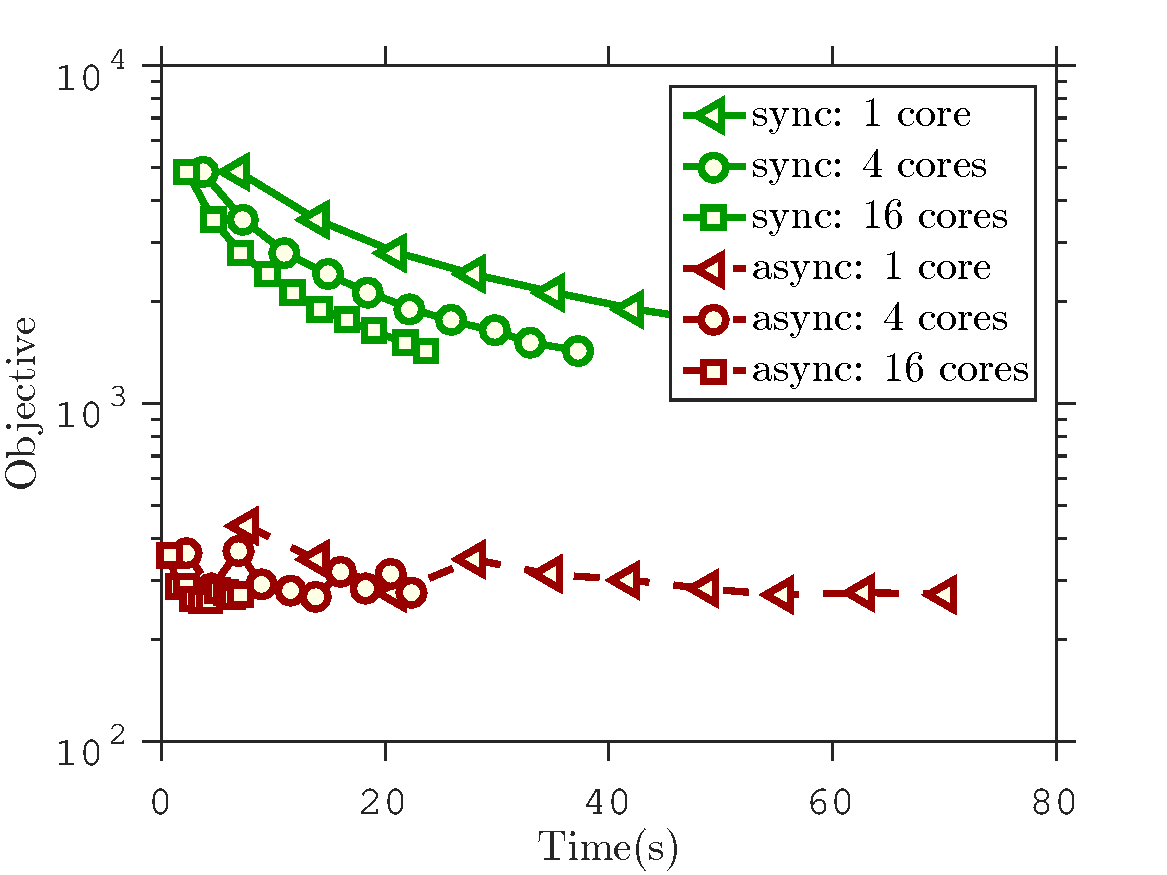
\includegraphics[width=\textwidth]{./figs/news20_obj}
                \caption{dataset ``news20''}
        \end{subfigure}
        ~~
        \begin{subfigure}[b]{0.4\textwidth}
                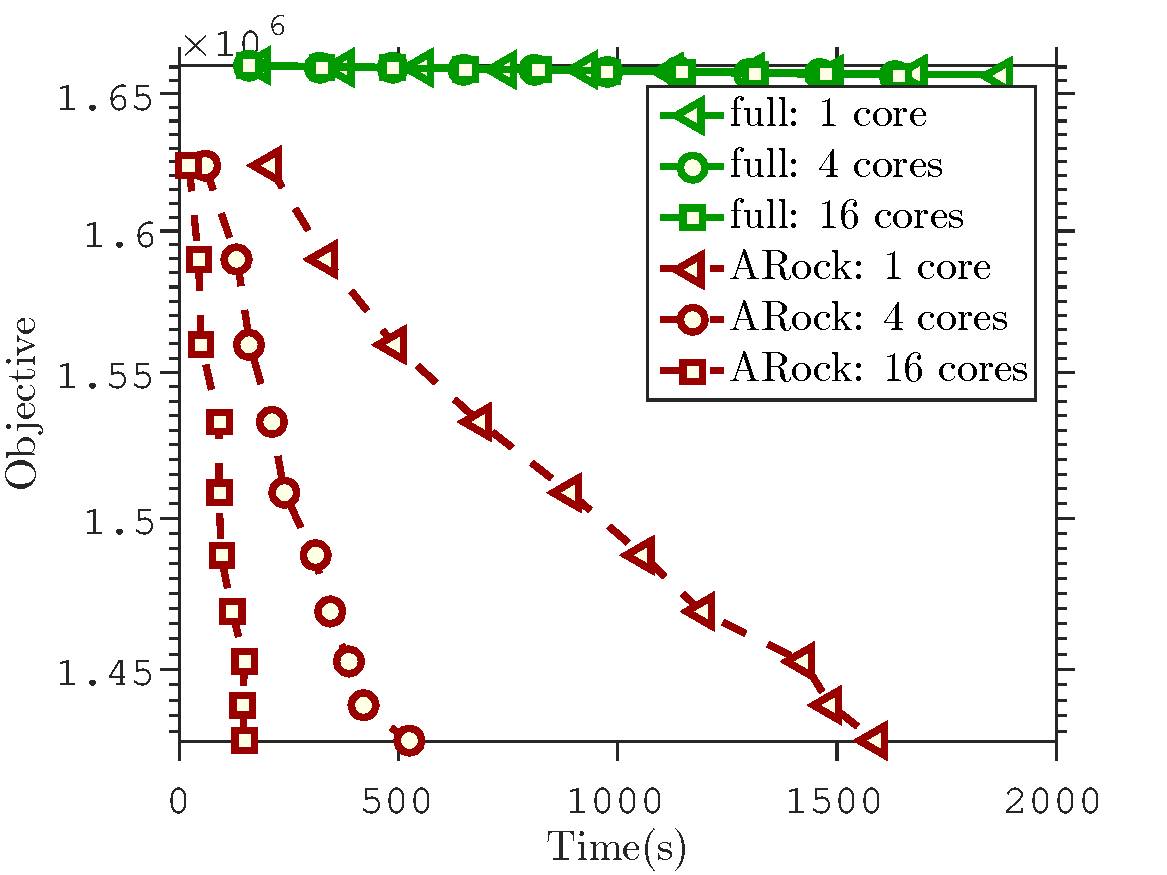
\includegraphics[width=\textwidth]{./figs/url_obj}
                \caption{dataset ``url''}
        \end{subfigure} 
        \caption{Objective vs wall clock time.}\label{fig:log_reg_obj}
\end{figure}
\begin{figure}[!h]
        \centering
       \begin{subfigure}[b]{0.35\textwidth}
                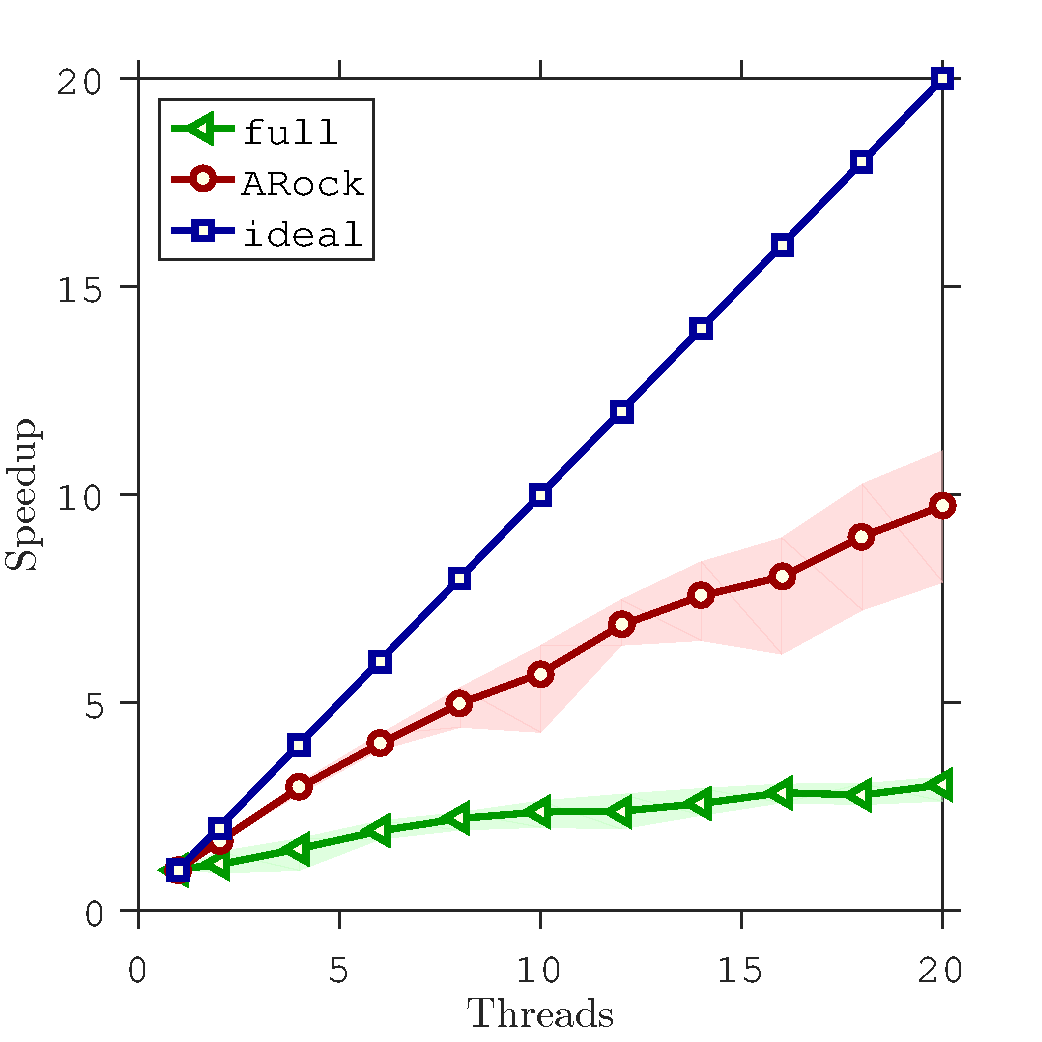
\includegraphics[width=\textwidth]{./figs/news20_speedup}
                \caption{dataset ``news20''}
        \end{subfigure}
        ~~
        \begin{subfigure}[b]{0.35\textwidth}
                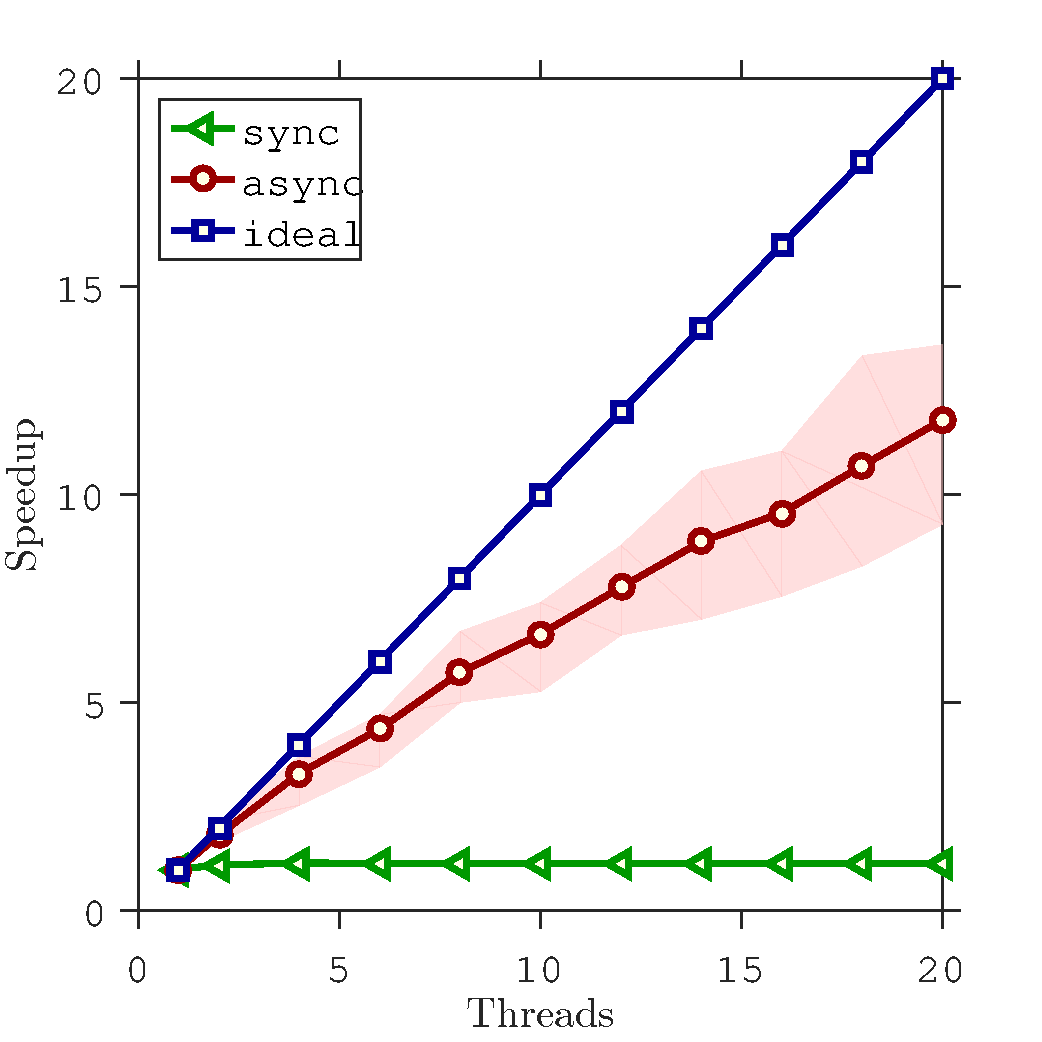
\includegraphics[width=\textwidth]{./figs/url_speedup}
                \caption{dataset ``url''}
        \end{subfigure}        
        \caption{Speedup vs number of threads. The solid lines represent mean speedup across 10 different runs. The shaded regions represent the lower and upper bounds of speedup for the 10 runs.}\label{fig:log_reg_speedup}
\end{figure}
